\chapter{Automatisation du processus d'investigation}
\label{Automatisation du processus d'investigation}
\thispagestyle{fancy}
Lorsqu'une error name est révélée (partie \ref{Introduction:Expression du besoin:Hiérarchisation des erreurs}) durant le Filtering test, de nombreuses données sont enregistrées dans un fichier journal (que l'on retrouve plus souvent sous le terme anglais de fichier "log".) Une analyse poussée de ces informations permet de déterminer la root cause liée à l'error name (partie \ref{Introduction:Expression du besoin:Hiérarchisation des erreurs}). Afin d'automatiser ce processus d'analyse, on s'appuie sur l'utilisation d'algorithmes d'apprentissage automatique. 

\section{Architecture High Level du système proposé}
\label{Automatisation du processus d'investigation: Achitecture High Level du système proposé}
L'architecture haut niveau de la solution que l'on propose est composée de deux couches: une couche "root cause" et une couche "error name".
\begin{description}
	\item [Couche root cause] La couche root cause permet de détecter la présence d'une root cause dans l'exemple que l'on analyse.
	\item [Couche error name] La couche error name est constituée d'un ensemble de couches root cause, de telle manière que lorsqu'un fichier historique est mis en entrée du système, l'ensemble des couches root cause sont activées. Ainsi, le système recherche la présence de chaque root cause connue dans l'exemple étudié. On obtient en sortie de la couche error name le nom de la root cause ayant la plus forte probabilité d'avoir été reconnue.
\end{description} 

\subsubsection{Exemple de mise en place  d'une couche error name et de ses couches root cause}.
Afin de présenter de manière plus concrète l'architecture  haut niveau de notre solution, on soumet un exemple de mise en place d'une architecture de détection et son utilisation . \\

\paragraph{Mise en place du système de détection / Apprentissage}
On souhaite dans un premier temps mettre en place l'architecture permettant de détecter la cause (root cause) ayant entrainé la chute du robot lors du Filtering test (error name). Cette étape consiste en 

\begin{figure}[h]
	\centering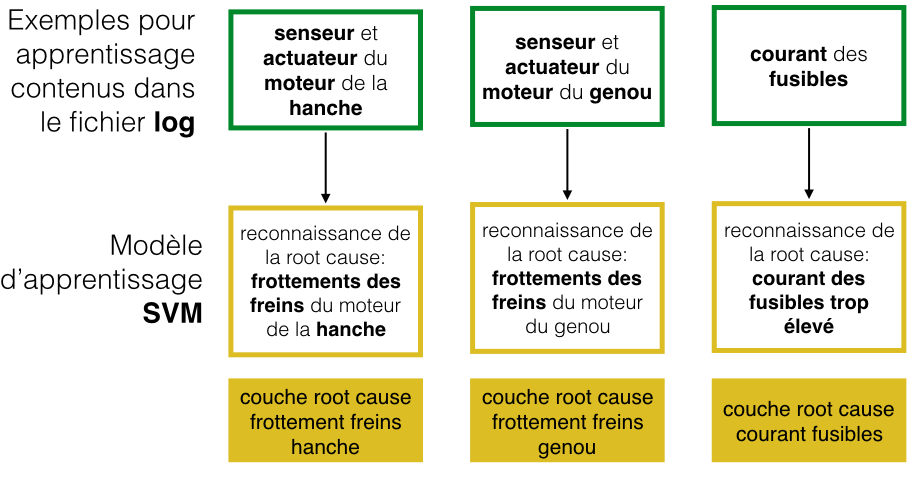
\includegraphics[height=6.5cm]{images/synoptique_root.png}
	\caption[Synoptique haut niveau de la couche root cause]{Synoptique haut niveau de la couche root cause. Le schéma de la couche root cause reprend celui du fonctionnement High Level de l'apprentissage automatique (figure \ref{fig:Schéma fonctionnel haut niveau du Machine Learning}). En effet, le système doit détecter la présence d'une root cause, à partir de l'analyse du fichier log à l'entrée du système. Pour cela, l'algorithme est préalablement entraîne à partir d'exemples de fichiers logs labellisés.}
	\label{fig:synoptique haut niveau de la solution proposée: couche root cause}
\end{figure}

\begin{figure}[h]
	\centering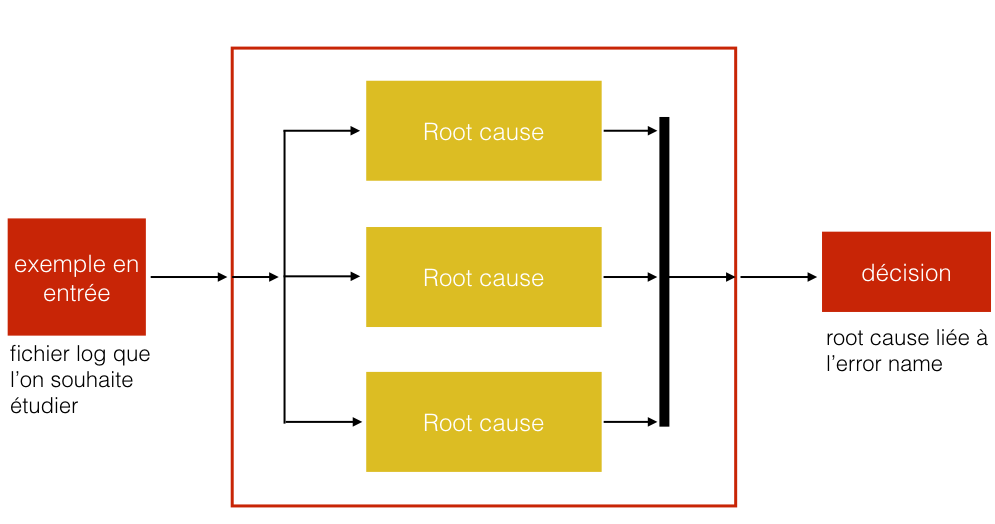
\includegraphics[height=6.5cm]{images/synoptique_error.png}
	\caption[Synoptique haut niveau de la couche error name]{Synoptique haut niveau de la couche error name. La couche error name contient plusieurs couches root cause. On met en entrée du système le fichier log que l'on souhaite analyser, puis chaque couche root cause va détecter la présence de la root cause à laquelle elle est rattachée. On obtient en sortie de la couche error name la root cause  ayant la plus forte probabilité d'avoir été reconnue.}
	\label{fig:synoptique haut niveau de la solution proposée: couche error name}
\end{figure}

On s'intéressera plus particulièrement à la couche "root cause" dans le reste de notre étude de l'architecture High Level, car elle contient l'ensemble du traitement et de l'analyse des données.

\subsection{Les exemples}
\label{Automatisation du processus d'investigation: Achitecture High Level du système proposé: Les exemples}

\subsection{Le modèle d'apprentissage}
\label{Automatisation du processus d'investigation: Achitecture High Level du système proposé: Le modèle d'apprentissage}

\subsection{La décision}
\label{Automatisation du processus d'investigation: Achitecture High Level du système proposé: La décision}



\section{Solutions techniques testées}
\label{Automatisation du processus d'investigation: Solutions techniques testées}




\section{Solution technique proposée}
\label{Automatisation du processus d'investigation: Solution technique proposée}

